% Especificaciones del tamaño de letra, tamaño de hoja, márgenes, librerias, etc.
\documentclass[12pt, letterpaper]{article}
\usepackage[english]{babel}
\usepackage{fancyhdr}
\usepackage[utf8]{inputenc}
\usepackage[T1]{fontenc}
\usepackage{amsmath}
\usepackage{graphicx}
\usepackage{subcaption}
\usepackage[hidelinks]{hyperref}
\usepackage{url}
\usepackage{amssymb}
\usepackage{float}
\usepackage[margin=1in]{geometry}
\renewcommand{\baselinestretch}{1.5}

% Enlace Bibliografía
\usepackage{csquotes}
\usepackage[notes,backend=biber]{biblatex-chicago}
\addbibresource{referencias.bib}

% Titulo, autores, fecha.
\title{Tarea \#5: Uso de la Gráfica Psicrométrica}
\author{Carlos Vásquez \and 1155057}
\pagestyle{fancy}
\fancyhf{}
\rhead{Carlos Vásquez}
\lhead{Gráfica Psicrométrica}
\rfoot{\thepage}


% Inicio del documento
\begin{document}
\maketitle
\subsection*{Resuelva el siguiente problema utilizando la gráfica psicrométrica.}
Aire húmedo a 33 ºC, 1 atm y 30\% de humedad relativa fluye a través de unos serpentines de enfriamiento a 0.47 $\frac{m^3}{s}$. El aire sale a 15 ºC. Determine a) la humedad relativa a la salida, b) la transferencia de calor desde el aire, en kJ sobre kg de aire seco, c) el flujo másico del aire seco, en kg de aire seco sobre segundo, y d) la tasa de transferencia de calor desde el aire, en kW.\\
\textbf{Solución}\\
a) Dado que nuestro aire se encuentra a una presión de 1 atmósfera, podemos utilizar los datos brindados para encontrar la humedad relativa a la salida.

\begin{figure}[H]
	\centering
	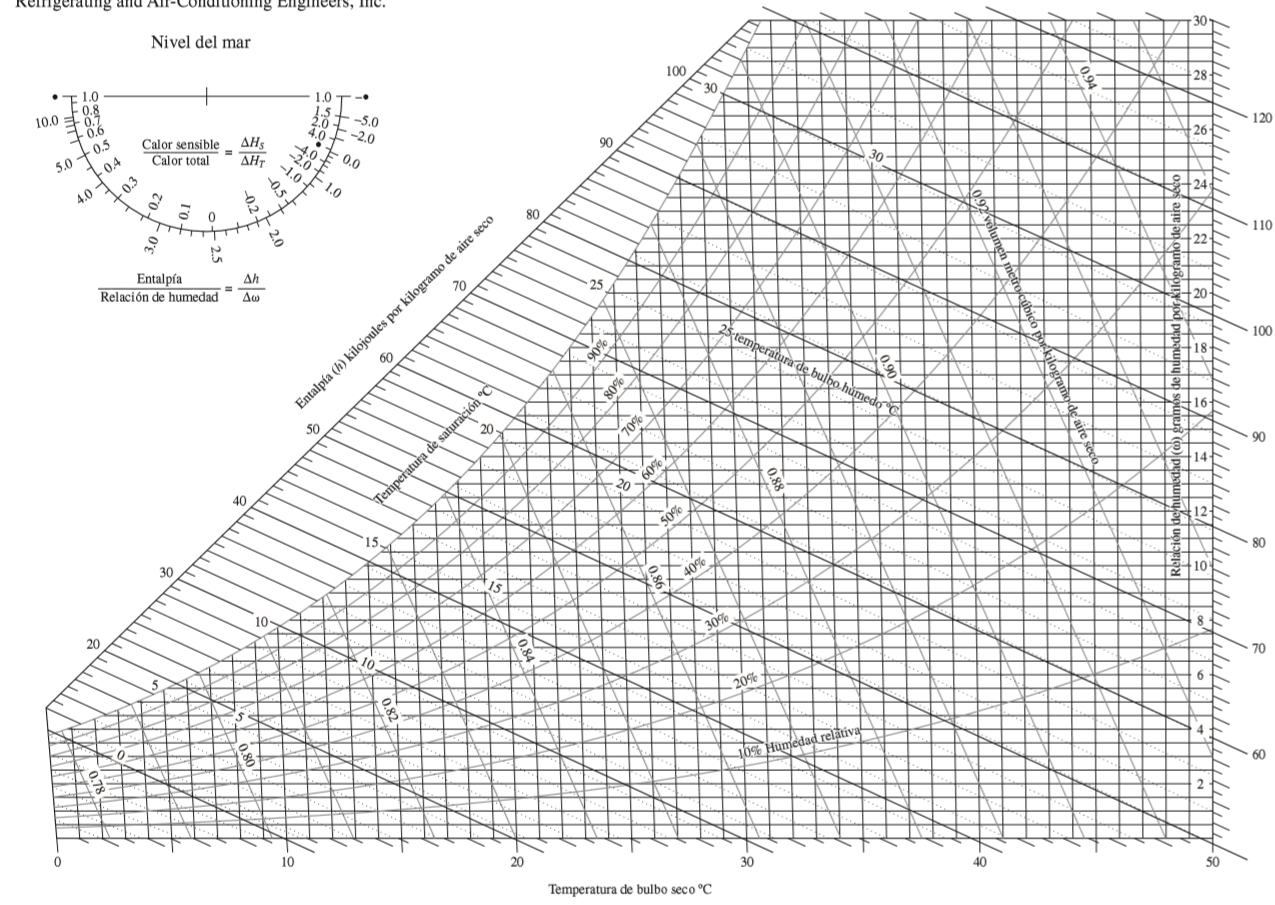
\includegraphics[width=0.6\textwidth]{1.png}
	\caption{Gráfica psicrométrica utilizada para resolver este ejercicio.}
\end{figure}
Si analizamos detenidamente la gráfica, podemos observar que a una temperatura de 33 ºC y una humedad relativa $\phi_1 = 30\%$ tenemos una humedad específica $\omega_1 = 9.5 \frac{g\ de\ vapor}{g\ de\ aire\ seco} = 0.0095 \frac{kg\ vapor}{kg\ aire\ seco}$. Dado que en procesos de calentamiento y enfriamiento simple la humedad específica se mantiene constante, podemos decir que $\omega_1 = \omega_2$, por lo que podemos utilizar este dato para encontrar la humedad relativa al final del proceso. Ya que tenemos nuestra temperatura final, $T_2 = 15\ ºC$, podemos utilizar la gráfica para encontrar la humedad relativa correspondiente a esa temperatura y a esa humedad específica.
\begin{figure}[H]
	\centering
	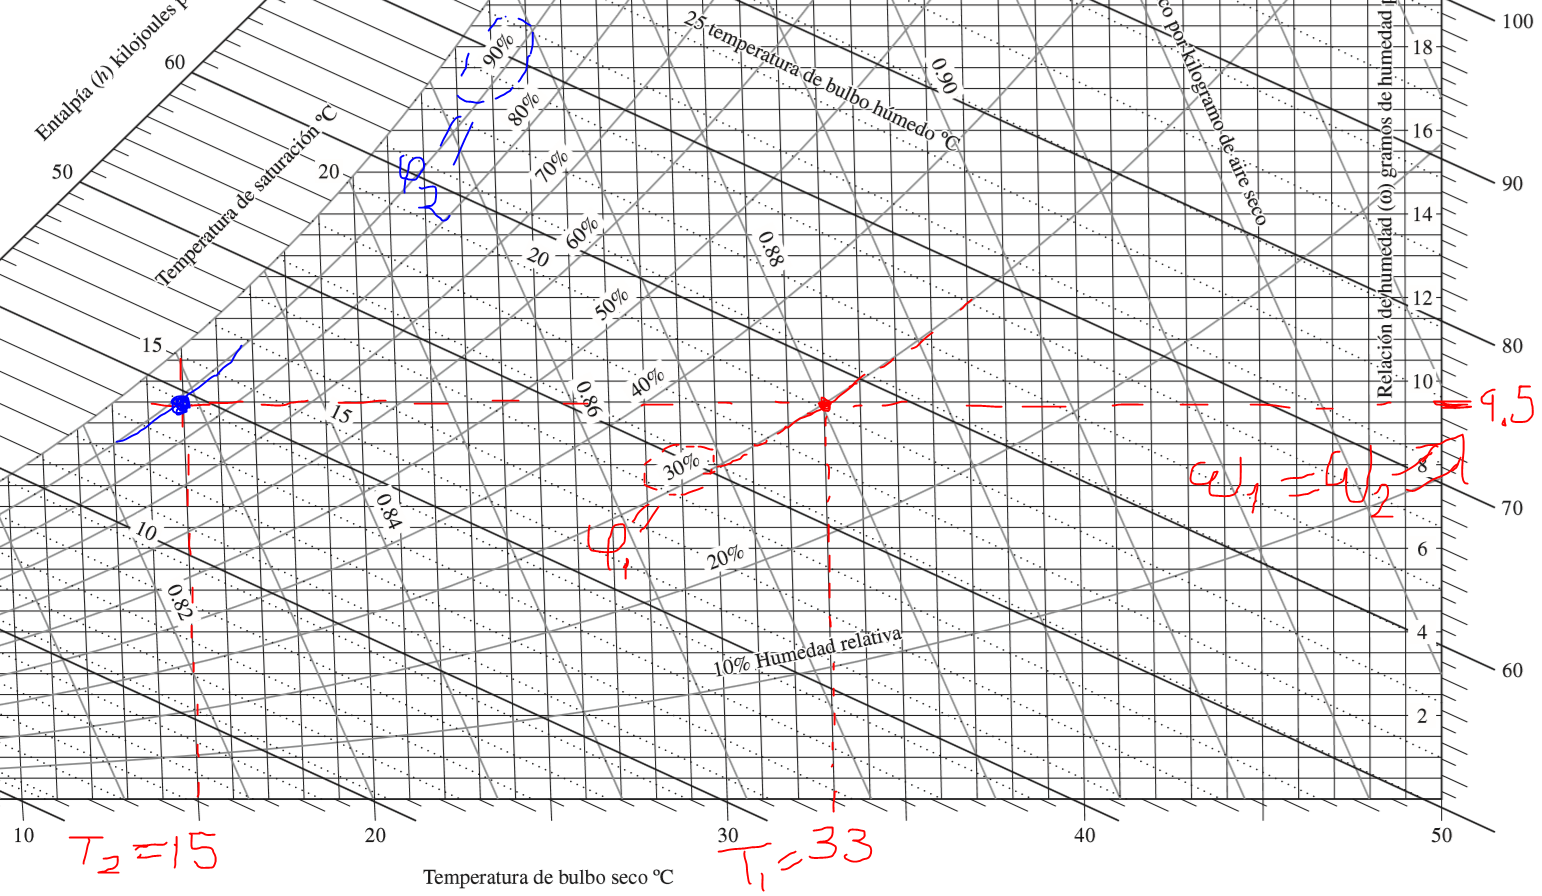
\includegraphics[width=\textwidth]{2.png}
	\caption{Método por el cual hallamos $\phi_2$}
\end{figure}

Por lo tanto, podemos estimar gracias a la gráfica psicrométrica que la humedad relativa al final del proceso será
\begin{equation}
	\boxed{\phi_2 = 90\%}
\end{equation}
Esta humedad relativa es menor a 100\%. En este caso el aire no sale saturado debido a que no se alcanza a llegar a la temperatura del punto de rocía, la cual es aproximadamente 13 ºC con las condiciones a las que se encuentra el aire que estamos analizando. Si se hubiese llegado a la temperatura del punto de rocío entonces hubiésemos obtenido un aire saturado y la humedad relativa hubiese sido 100\%.
\\

b) La transferencia de calor que se nos solicita es desde el aire al ambiente, en otras palabras, dado que es un proceso de enfriamiento, podemos calcular el calor de \textit{salida} como
\begin{equation}
	q_{out} = h_1 - h_2
\end{equation}
Y dado que conocemos las condiciones iniciales y finales de nuestro proceso, entonces podemos obtener las entalpías mencionadas anteriormente para calcular el calor de salida.
\begin{figure}[H]
	\centering
	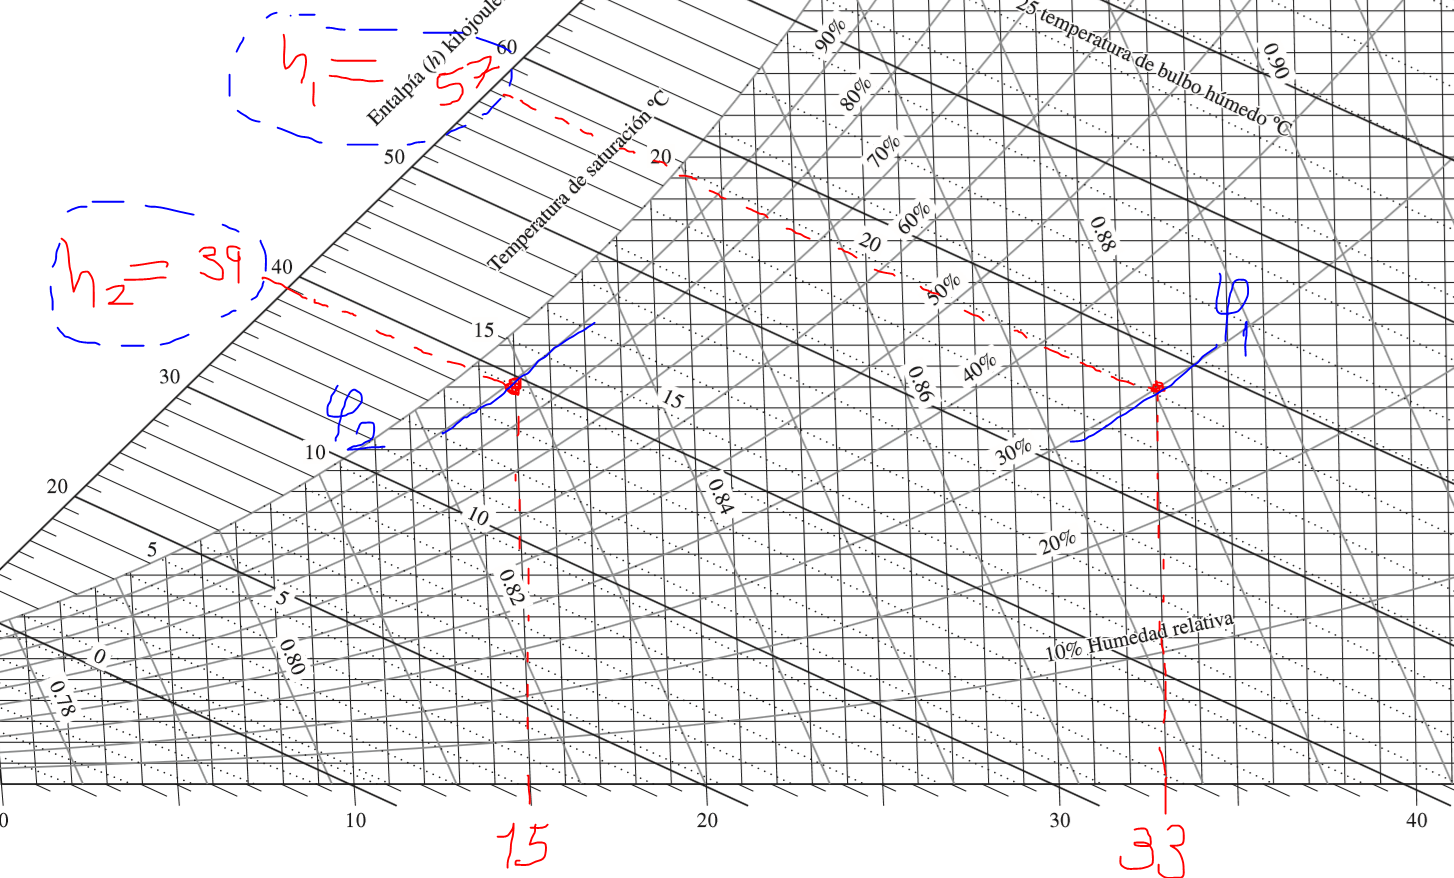
\includegraphics[width=\textwidth]{3.png}
	\caption{Estimación de las entalpías $h_1$ y $h_2$.}
\end{figure}
Como podemos observar en la figura 3, las entalpías son, aproximadamente, $h_1 = 57 \frac{kJ}{kg\ aire\ seco}$ y $h_2 = 39 \frac{kJ}{kg\ aire\ seco}$. Por tanto, el calor de salida será

\begin{equation}
	\boxed{\begin{split}
		q_{out} &= (57 \frac{kJ}{kg\ aire\ seco}) - (39 \frac{kJ}{kg\ aire\ seco})\\
		q_{out} &= 18 \frac{kJ}{kg\ aire\ seco}
	\end{split}}
\end{equation}

c) Para encontrar el flujo másico de nuestro fluido debemos encontrar el volumen específico en el estado inicial. Ya que tenemos el flujo volumétrico, el flujo másico es la relación

\begin{equation}
	\dot m_a = \frac{\dot V}{\nu_1}
\end{equation}

Para encontrar el volumen específico bastará con ver la gráfica psicrométrica y estimarlo.

\begin{figure}[H]
	\centering
	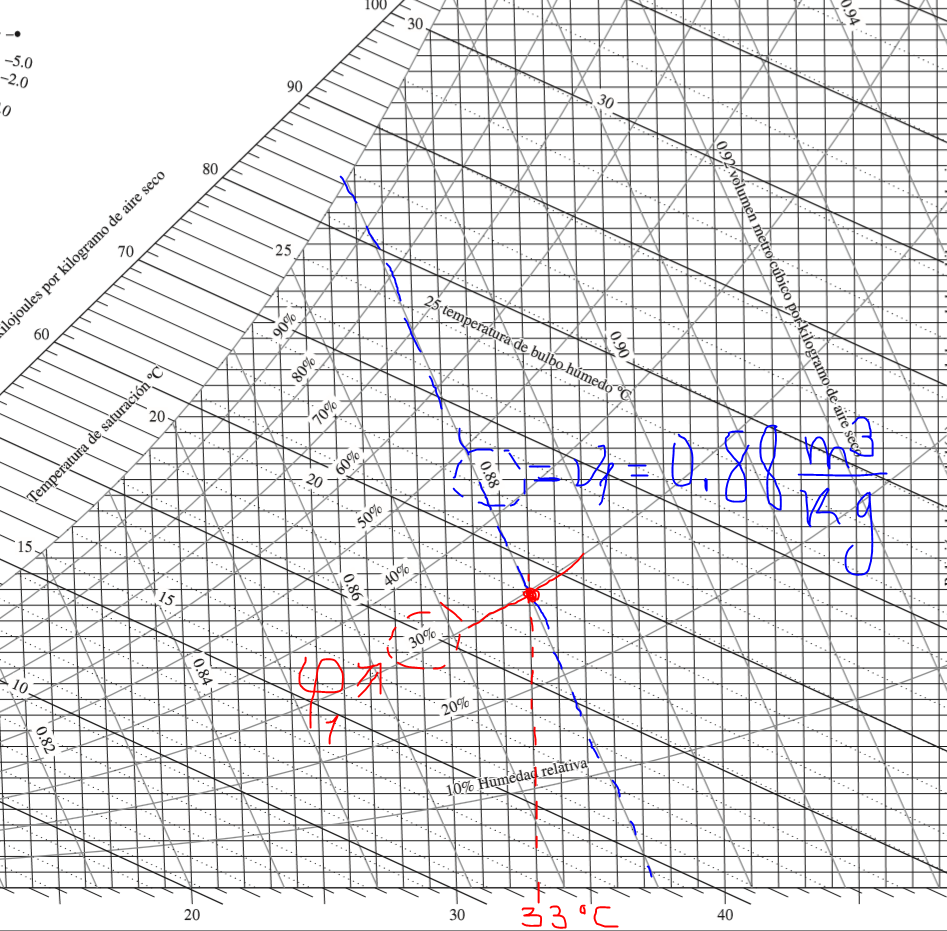
\includegraphics[width=\textwidth]{4.png}
	\caption{Estimación de $\nu_1$.}
\end{figure}

Gracias a la gráfica nos percatamos que el volumen específico es aproximadamente $\nu_1 = 0.88 \frac{m^3}{kg\ aire\ seco}$. Con esto es posible calcular el flujo másico.

\begin{equation}
	\boxed{
	\begin{split}
		\dot m_a &= \frac{0.47 \frac{m^3}{s}}{0.88 \frac{m^3}{kg\ aire\ seco}}\\
		\dot m_a &= 0.5341 \frac{kg}{s}
	\end{split}}
\end{equation}

d) Finalmente, para calcular la tasa de transferencia de calor la podemos obtener mediante los datos que ya hemos calculado. La tasa de transferencia de calor la podemos expresar como

\begin{equation}
	\begin{split}
		\dot Q_{out} &= \dot m_a (h_1 - h_2)\\
		\dot Q_{out} &= \dot m_a q_{out}
	\end{split}
\end{equation}

Por tanto, con los datos obtenidos anteriormente para $q_{out}$ y $\dot m_a$, la tasa de transferencia de calor, $\dot Q_{out}$ será

\begin{equation}
	\boxed{
	\begin{split}
		\dot Q_{out} &= (0.5341 \frac{kg}{s})(18 \frac{kJ}{kg\ aire\ seco})\\
		\dot Q_{out} &= 9.6136\ kW
	\end{split}}
\end{equation}
%%%%%  Bib
\renewcommand\refname{Referencias}
\printbibliography
\end{document}
